\documentclass[12pt]{article}
\usepackage[spanish]{babel}
\usepackage[utf8]{inputenc}
\usepackage{graphicx}
\usepackage{hyperref}
\usepackage{booktabs}
\usepackage{multirow}
\usepackage{amsmath}
\usepackage{float}
\usepackage[document]{ragged2e}
\usepackage{microtype}
\addto\captionsspanish{%
  \renewcommand{\tablename}{Tabla}%
}

\usepackage[a4paper, margin=2.5cm]{geometry}

% Configuración de encabezado
\usepackage{fancyhdr}
\pagestyle{fancy}
\fancyhf{}
\lhead{Detección de anomalías en series temporales multivariadas con aprendizaje por refuerzo}
\rfoot{Página \thepage}

\title{
    \vspace{-2cm}
    \normalsize \textbf{Universidad de Buenos Aires} \\
    \textbf{Laboratorio de Sistemas Embebidos} \\
    \textbf{Especialización en Inteligencia Artificial} \\
    \vspace{0.5cm}
    {Trabajo Práctico Final} \\
    \vspace{1cm}
    \Large \textbf{Detección de anomalías en series temporales multivariadas con aprendizaje por refuerzo} \\
    \vspace{1cm}
    \large Docente: Esp. Ing. Miguel Augusto Azar
    \vspace{1cm}
}
\author{
    Matías A. Marando
    \vspace{1cm}
}
\date{\today}

\begin{document}
\justifying
\maketitle

%%%%%%%%%%%%%%%%%%%%%%%%%%%%%%%%%%%%%%%%%%%%%%%%%%%%%%%%%%%%%%%%%%%%%%%%

\begin{abstract}
Este trabajo presenta un enfoque híbrido para la detección de anomalías en series temporales multivariadas (MTS) sintéticas, combinando un autoencoder LSTM para la generación de puntuaciones de anomalía y un agente de Q-Learning para la clasificación binaria de las MTS como normales o anómalas.
Se entrena un autoencoder LSTM para aprender la representación de datos normales, y su error de reconstrucción se utiliza como una métrica de anomalía.
Posteriormente, un agente de Q-Learning es entrenado para tomar decisiones de clasificación basándose en características extraídas de estas curvas de anomalía.
Se explora la representación de estados multidimensionales para el agente de Q-Learning y se realiza Grid Search para optimizar sus hiperparámetros y esquemas de recompensa.
Los resultados demuestran la efectividad del enfoque híbrido y la mejora en el rendimiento de la detección de anomalías al optimizar el agente de Q-Learning.
\end{abstract}

%%%%%%%%%%%%%%%%%%%%%%%%%%%%%%%%%%%%%%%%%%%%%%%%%%%%%%%%%%%%%%%%%%%%%%%%

\newpage
\section{Introducción}
\label{sec:intro}

La detección de anomalías en series temporales es un campo crítico con aplicaciones en diversas áreas, como la monitorización de sistemas, la ciberseguridad, la detección de fraudes y el mantenimiento predictivo. Una anomalía, en este contexto, se refiere a un patrón que no se ajusta a un comportamiento esperado de los datos, lo que a menudo indica un evento inusual o problemático. Las series temporales multivariadas (MTS), que consisten en múltiples variables que evolucionan a lo largo del tiempo, presentan desafíos adicionales debido a la complejidad de las interdependencias entre las variables.

Tradicionalmente, la detección de anomalías en series temporales se ha abordado con métodos estadísticos o basados en reglas.
Sin embargo, la creciente complejidad y volumen de los datos han impulsado la adopción de técnicas de aprendizaje automático, particularmente las redes neuronales profundas.
Los autoencoders, por ejemplo, son herramientas potentes para aprender representaciones compactas de datos normales y detectar anomalías basándose en errores de reconstrucción elevados.

Este trabajo explora la integración de un autoencoder LSTM con un algoritmo de Aprendizaje por Refuerzo (RL), específicamente Q-Learning, para mejorar la clasificación de anomalías en MTS.
Mientras que el autoencoder se encarga de generar una puntuación de anomalía para cada serie temporal, el agente de Q-Learning aprende una política óptima para clasificar estas series como normales o anómalas, adaptándose a diferentes criterios de rendimiento definidos por esquemas de recompensa.
La combinación busca aprovechar la capacidad del autoencoder para modelar la normalidad y la habilidad del Q-Learning para aprender políticas de decisión complejas en un entorno dinámico.

%%%%%%%%%%%%%%%%%%%%%%%%%%%%%%%%%%%%%%%%%%%%%%%%%%%%%%%%%%%%%%%%%%%%%%%%

\bigskip
\section{Metodología}
\label{sec:metodologia}

La metodología propuesta para la detección de anomalías en series temporales multivariadas se divide en varias etapas clave: generación de datos sintéticos, entrenamiento de un autoencoder LSTM para la puntuación de anomalías, y el diseño y entrenamiento de un agente de Q-Learning para la clasificación final.

\subsection{Generación de datos sintéticos}
Para simular un entorno controlado y reproducible, se generaron series temporales multivariadas sintéticas.
Cada MTS consta de $N$ variables (en este caso, $3$) señales, cada una generada como una combinación de patrones sinusoidales y de rampa con ruido gaussiano.
Este enfoque permite crear datos normales con variabilidad controlada.

Para simular anomalías, se implementó un mecanismo de inyección de anomalías.
En un porcentaje de las MTS generadas, se introducen cambios abruptos en una de las variables durante un corto período de tiempo.
Estos cambios se realizan alterando el valor de la señal a un valor significativamente desviado de su media y desviación estándar, simulando picos o caídas inesperadas.
Cada MTS anómala se etiqueta con un $1$, mientras que las normales se etiquetan con un $0$.

\subsection{Autoencoder LSTM}
Un autoencoder LSTM fue seleccionado para aprender la representación de las series temporales normales y generar una puntuación de anomalía.

\begin{itemize}
    \item Arquitectura: el autoencoder consiste en un encoder LSTM que comprime la secuencia de entrada en un espacio latente y un decoder LSTM que intenta reconstruir la secuencia original a partir de esta representación latente.
    \item Entrenamiento: el modelo se entrena exclusivamente con series temporales multivariadas normales.
    \item Puntuación de anomalías: después del entrenamiento, para cada MTS, se calcula el error de reconstrucción (MSE) entre la entrada original y su reconstrucción por el autoencoder. Esta secuencia de errores de MSE a lo largo del tiempo para cada MTS se denomina curva de anomalía.
    \item Umbral fijo: para establecer una línea base, se calcula un umbral de anomalía a partir de la distribución de los errores de reconstrucción del conjunto de entrenamiento normal (percentil 99.5). Cualquier MTS cuyo error de reconstrucción máximo supere este umbral se clasifica como anómala.
\end{itemize}

\subsection{Agente de Q-Learning}
El agente de Q-Learning aprende a clasificar las MTS como normales o anómalas basándose en las curvas de anomalía generadas por el autoencoder.

\begin{itemize}
    \item \textbf{Estado ($S$)}: el estado del agente se construye a partir de características estadísticas extraídas de la curva de anomalía de una MTS dada.
    Estas características pueden incluir el valor máximo ($\max$), la media ($\mu$), la desviación estándar ($\sigma$), la mediana y/o el rango.
    Para la discretización del espacio de estados, se utilizan $N$ estados (por ejemplo, $2, 4$ u $8$) bins para cada característica seleccionada.
    Si se seleccionan múltiples características (e.g., 'max' y 'mean'), el estado se convierte en un índice único que representa la combinación discreta de estos valores.
    Esto permite una representación de estado multidimensional.
    \item \textbf{Acciones ($A$)}: el agente tiene dos acciones posibles:
    \begin{itemize}
        \item Acción 0: clasificar la MTS como normal.
        \item Acción 1: clasificar la MTS como anómala.
    \end{itemize}
    \item \textbf{Recompensa ($R$)}: La recompensa se define en función de la acción elegida por el agente y la etiqueta real de la MTS. Se exploran diferentes esquemas de recompensa para guiar el aprendizaje del agente:
    \begin{itemize}
        \item \texttt{Balanced}: recompensas moderadas para TP y TN, penalizaciones para FP y FN.
        \item \texttt{Conservative}: prioriza evitar Falsos Positivos (FP) y Falsos Negativos (FN) con penalizaciones más altas.
        \item \texttt{Aggressive}: prioriza la detección de anomalías (TP) con recompensas más altas para TP y penalizaciones para FN.
    \end{itemize}
    Un ejemplo de esquema de recompensa (\texttt{Balanced}) es: $TP = 50$, $TN = 25$, $FP = -25$, $FN = -100$.
    \item \textbf{Función de Valor-Acción ($Q(S,A)$)}: el agente mantiene una tabla Q, que almacena el valor esperado de tomar una acción $A$ en un estado $S$. La tabla Q se inicializa con ceros.
    \item \textbf{Política de Exploración-Explotación}: se utiliza una política $\epsilon$-greedy.
    Con probabilidad $\epsilon$, el agente elige una acción aleatoria (exploración); de lo contrario, elige la acción con el valor Q más alto para el estado actual (explotación). El valor de $\epsilon$ decae exponencialmente con cada episodio de entrenamiento, comenzando en $1.0$ y disminuyendo hasta un mínimo de $0.1$.
    \item \textbf{Actualización de la tabla Q}: la tabla Q se actualiza utilizando la siguiente regla:
    $$Q(S_t, A_t) \leftarrow Q(S_t, A_t) + \alpha (R_{t+1} - Q(S_t, A_t))$$
    donde $\alpha$ es la tasa de aprendizaje y $R_{t+1}$ es la recompensa recibida.
    Esta forma de actualización es adecuada para problemas donde la decisión se toma en un solo paso y no hay una secuencia de estados subsiguientes que requieran un factor de descuento $\gamma$ para considerar futuras recompensas.
\end{itemize}

\subsection{Grid Search para Q-Learning}
Para optimizar el rendimiento del agente de Q-Learning se implementó un grid search sobre los siguientes hiperparámetros y configuraciones:
\begin{itemize}
    \item Número de estados: \texttt{[2, 4, 8]}
    \item Esquema de recompensa: \texttt{Balanced, Conservative, Aggressive}
    \item Combinaciones de características de estado: \texttt{['max'], ['max', 'std'], ['max', 'mean']}
\end{itemize}
Cada combinación de parámetros se entrena y evalúa, y se selecciona la combinación que maximiza una métrica de rendimiento compuesta.

%%%%%%%%%%%%%%%%%%%%%%%%%%%%%%%%%%%%%%%%%%%%%%%%%%%%%%%%%%%%%%%%%%%%%%%%

\bigskip
\section{Resultados}
\label{sec:resultados}

\subsection{Rendimiento de los modelos}
Se evaluaron tres enfoques de clasificación de anomalías en un conjunto de prueba compuesto por $90$ series normales y $10$ series anómalas.

\begin{enumerate}
    \item LSTM (umbral fijo): este método utiliza directamente el umbral calculado por el autoencoder.
    \item Agente RL base: un agente de Q-Learning entrenado con parámetros por defecto.
    \item Mejor agente RL (grid search): el agente de Q-Learning con la combinación de hiperparámetros y características de estado que arrojó el mejor rendimiento en grid search.
\end{enumerate}

La figura \ref{fig:comparacion_modelos} resume las métricas de rendimiento clave para cada modelo.

\begin{figure}[H]
\centering
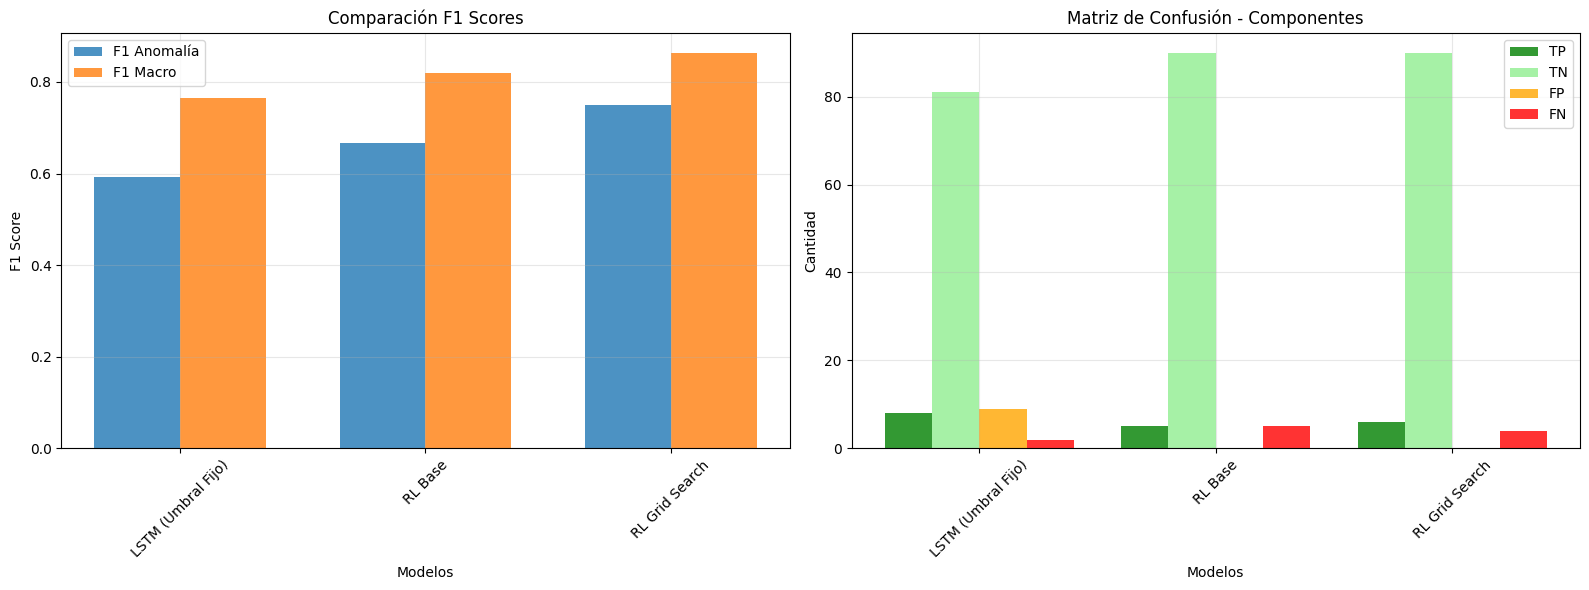
\includegraphics[width=1\textwidth]{media/metrics_comparison.png}
\caption{Gráficas comparativas del rendimiento de los modelos.}
\label{fig:comparacion_modelos}
\end{figure}

Análisis de los resultados:

\begin{itemize}
    \item LSTM (umbral fijo): muestra un buen recall para anomalías (0.800), pero a costa de una precisión muy baja (0.471) debido a un alto número de falsos positivos. Su F1-score para anomalías (0.593) y su accuracy general (0.890) son los más bajos de la comparativa.
    \item Agente RL base: al utilizar un agente RL con parámetros por defecto (características \texttt{['max', 'std']}), se eliminan por completo los falsos positivos, logrando una precisión perfecta. Sin embargo, esto se consigue sacrificando el recall (0.500), ya que clasifica incorrectamente la mitad de las anomalías reales.
    \item Mejor agente RL (grid search): el agente optimizado mantiene la precisión perfecta pero mejora el recall reduciendo los falsos negativos. Este equilibrio se traduce en el mejor rendimiento global.
\end{itemize}

\subsection{Gráfico de convergencia del agente RL}
La figura \ref{fig:rl_convergence} muestra el progreso del entrenamiento del agente de Q-Learning, incluyendo la convergencia de las recompensas y el decaimiento del valor de $\epsilon$.

\begin{figure}[H]
\centering
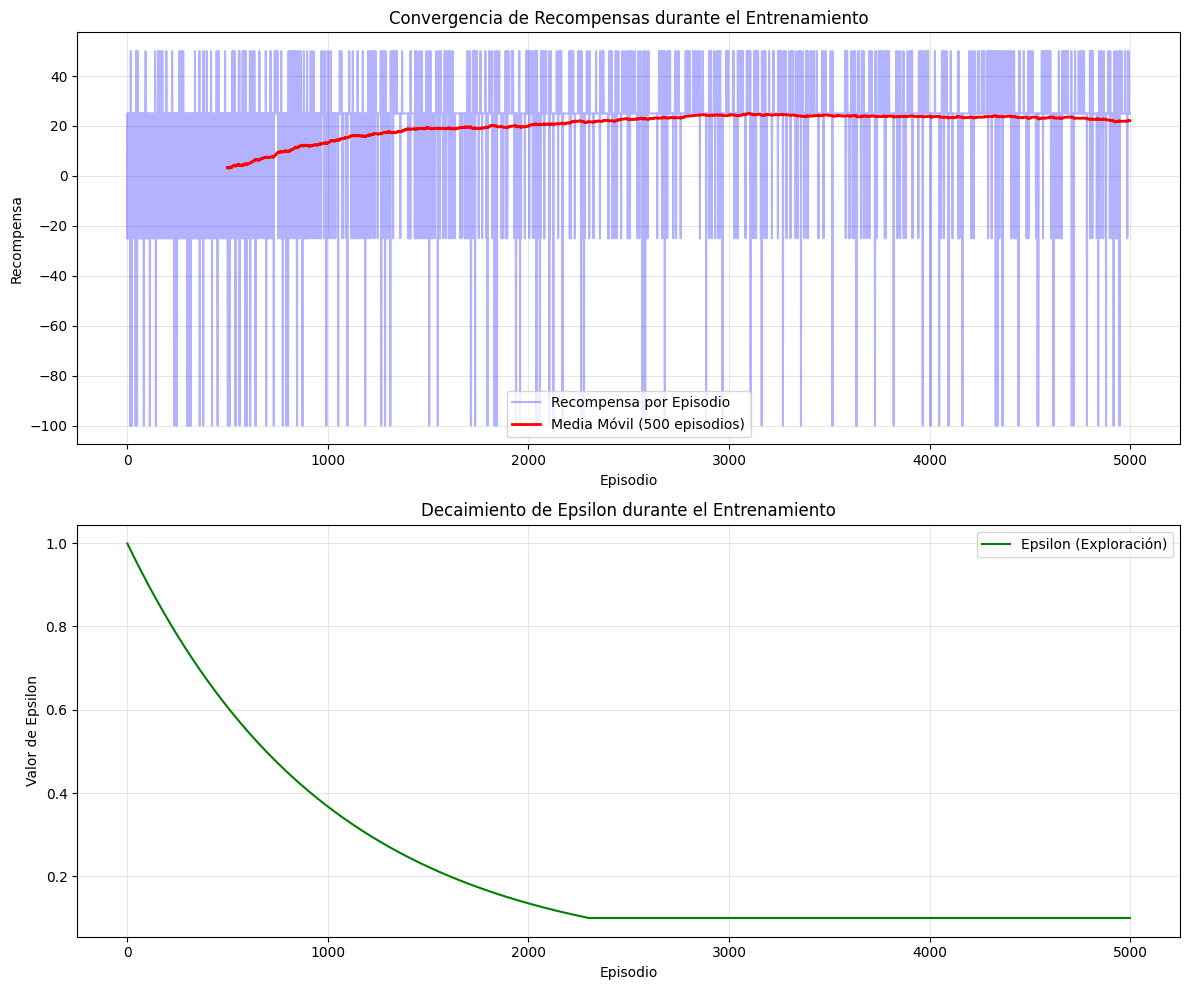
\includegraphics[width=1\textwidth]{media/rl_training.png}
\caption{Convergencia de recompensas y decaimiento de epsilon.}
\label{fig:rl_convergence}
\end{figure}

La curva de recompensa por episodio, suavizada con una media móvil, demuestra una tendencia ascendente y una eventual estabilización.
Esto indica que el agente está aprendiendo una política que maximiza la recompensa acumulada a lo largo del tiempo, es decir, está mejorando su capacidad para clasificar correctamente las MTS y evitar penalizaciones.

La curva de $\epsilon$ muestra una disminución gradual desde su valor inicial (1.0) hasta su valor mínimo (0.1).
Este comportamiento es crucial para el entrenamiento de RL, ya que permite que el agente explore el espacio de acciones al principio del entrenamiento (cuando $\epsilon$ es alto) y luego explote el conocimiento aprendido a medida que $\epsilon$ disminuye, lo que conduce a una política más estable y óptima.

\subsection{Ejemplos de clasificación}
Se visualizaron ejemplos de cada categoría de clasificación para entender el comportamiento de los modelos.
La figura \ref{fig:classification_example} muestra un caso donde el LSTM con umbral fijo falla mientras que los agentes RL logran una clasificación correcta.

\begin{figure}[H]
\centering
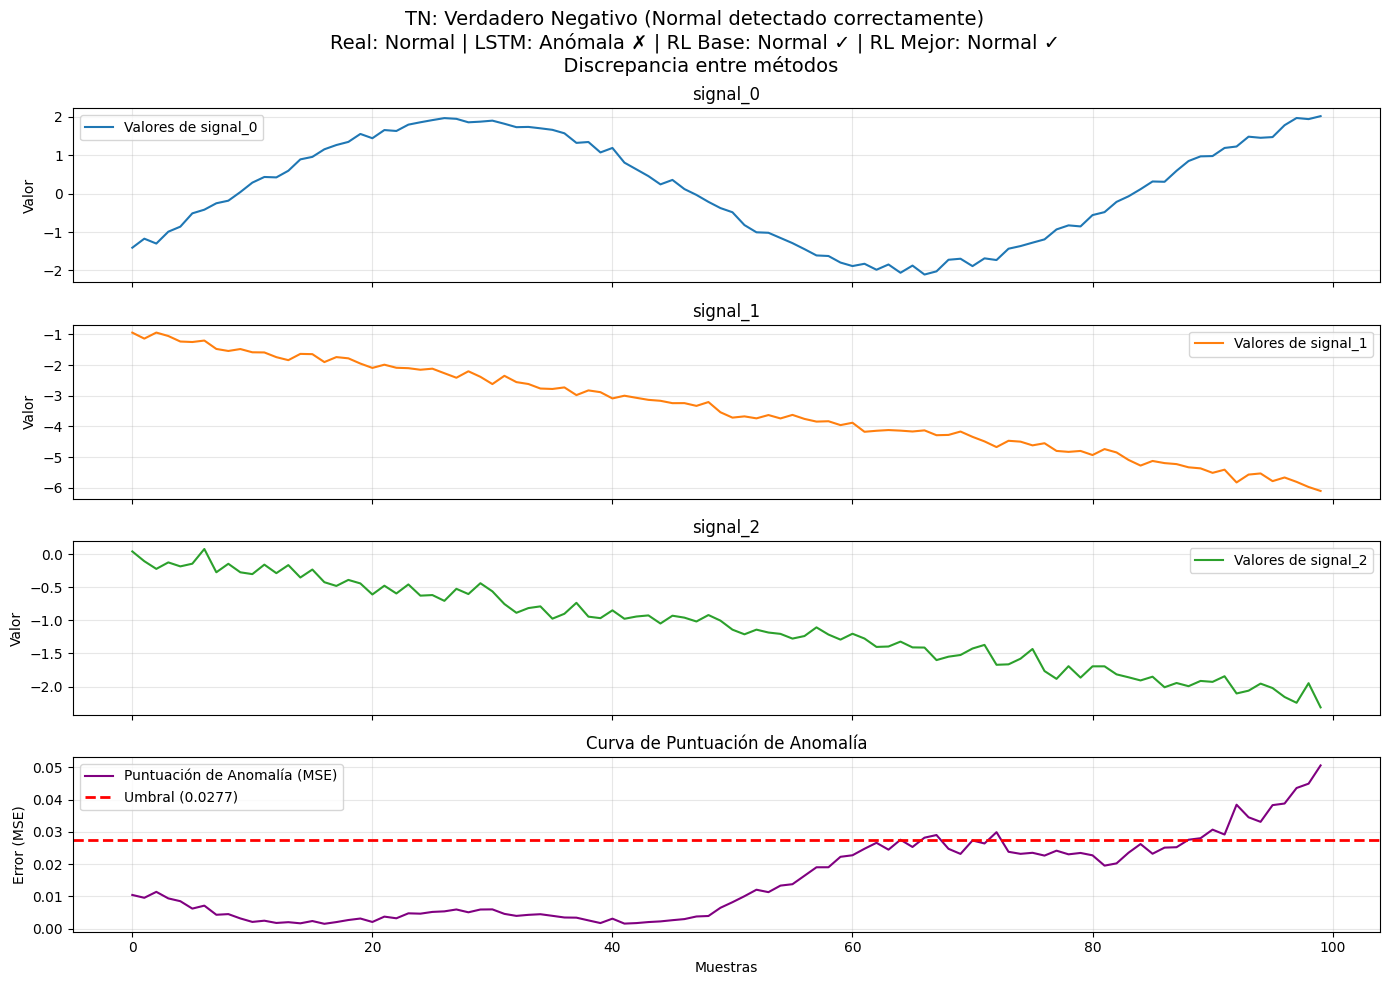
\includegraphics[width=1\textwidth]{media/classification_example.png}
\caption{Ejemplo de clasificación de los modelos.}
\label{fig:classification_example}
\end{figure}

%%%%%%%%%%%%%%%%%%%%%%%%%%%%%%%%%%%%%%%%%%%%%%%%%%%%%%%%%%%%%%%%%%%%%%%%

\bigskip
\section{Conclusiones}
\label{sec:conclusiones}

\subsection{Hallazgos clave}

\begin{itemize}
    \item La combinación de un Autoencoder LSTM para la puntuación de anomalías y un agente de Q-Learning para la clasificación final demostró ser un enfoque prometedor para la detección de anomalías en series temporales multivariadas. El autoencoder logra una representación efectiva de los datos normales, y su error de reconstrucción sirve como una señal robusta para la presencia de anomalías.
    \item El agente de Q-Learning, al aprender una política de clasificación basada en características de las curvas de anomalía, superó al método de umbral fijo del LSTM, especialmente en la reducción de falsos positivos y en la mejora del F1-score. Esto resalta la capacidad del aprendizaje por refuerzo para adaptarse a criterios de rendimiento complejos y tomar decisiones más matizadas que un umbral estático.
    \item La implementación de grid search fue fundamental para optimizar el rendimiento del agente de Q-Learning. La selección adecuada de parámetros resultaron en el mejor rendimiento general.
    \item Los gráficos de convergencia confirmaron que el agente de Q-Learning aprendió una política con recompensas que aumentan y se estabilizan a medida que disminuye la exploración.
\end{itemize}

\subsection{Trabajo futuro}

\begin{itemize}
    \item Aplicar el enfoque a conjuntos de datos de series temporales multivariadas reales de diversas fuentes (sensores industriales, tráfico de red, datos financieros) para validar su robustez y generalización.
    \item Explorar la detección de diferentes tipos de anomalías (contextuales, colectivas, de punto más sutiles) que puedan requerir representaciones de estado o arquitecturas de autoencoder más sofisticadas.
    \item Investigar el uso de algoritmos de Deep Reinforcement Learning (DRL), como Deep Q-Networks (DQN) o modelos Actor-Critic, que pueden manejar espacios de estados y acciones continuos o de alta dimensionalidad sin necesidad de discretización explícita.
\end{itemize}

%%%%%%%%%%%%%%%%%%%%%%%%%%%%%%%%%%%%%%%%%%%%%%%%%%%%%%%%%%%%%%%%%%%%%%%%

\newpage
\section*{Anexo}
El código completo se encuentra disponible en \url{https://github.com/mmarando/rl1}.

\end{document}
